\documentclass[11pt]{article}
% -----------------------------------------------------------------------------
% Results_analysis: preliminary analysis of the results of the final case study (MS CPENG-8674, major revision).
% Runs: Output/review29oct_fixed/KSVAE_fixed_03Nov-FINAL_7D_{1,3,5}KS_obs-fv_Gamma1.0_Ep1500 (5 modes).
% Figures: ./figures_results (copied from the K = 3 run). Extra statistics were computed from the saved
% predictions and the cached exact posteriors; no model was retrained.
% -----------------------------------------------------------------------------
\usepackage[a4paper,margin=2.3cm]{geometry}
\usepackage{amsmath,amssymb,bm}
\usepackage{graphicx}
\usepackage{booktabs,array}
\usepackage{xcolor}
\usepackage{caption}
\usepackage{enumitem}
\usepackage{titlesec}
\usepackage[colorlinks=true,linkcolor=red!70!black,citecolor=red!70!black,urlcolor=magenta]{hyperref}

\linespread{1.12}
\captionsetup{labelfont=bf,font=small,labelsep=colon}
\titleformat{\section}{\normalfont\sffamily\bfseries\large}{\thesection}{0.6em}{}
\titleformat{\subsection}{\normalfont\bfseries}{\thesubsection}{0.6em}{}
\setlist{itemsep=2pt,topsep=3pt}
\newcommand{\z}{\mathbf{z}}
\newcommand{\zb}[1]{z_{b,\mathrm{#1}}}

\title{\sffamily\bfseries Results analysis\\[4pt]
\large Preliminary analysis of the results of the final case study (MS CPENG-8674)}
\author{}
\date{3 November 2026 --- runs in \texttt{Output/review29oct\_fixed}}

\begin{document}
\maketitle

\section*{Main findings}
\begin{itemize}
\item On the 11 benchmarks, the VAE reproduces the exact (SMC) posteriors in both test sets: means within 0.010
(0.015 in test set B), standard deviations within 8\% (10\%), Frobenius error of the correlation matrices 0.13--0.26
(0.13--0.29). The errors with respect to the true values that remain are also present in the exact posteriors.
\item The equal-tailed 95\% coverage is 0.900 on test set A (0.946 with highest-density intervals). For the deck zones
the shortfall is explained by the design of the test set, which places two thirds of the parameters at the upper bound
of the prior: on the scenarios drawn from the prior, the deck zones reach 0.945. The bearings under-cover there too
(0.900), and so does the exact posterior of the same 120 structures (0.904, against 0.957 for the deck zones): the
cause is the likelihood, not the VAE. Its mode-shape term treats the as-built shape errors as independent across
sensors, but in modes 4 and 5 they are concentrated in the directions in which the bearings change the shapes, so the
likelihood over-weights the mode-shape evidence about the bearings (by a factor of about 1.6 in those modes).
\item The width of the posteriors follows the physics: the end zones, which store little strain energy, are the least
informed parameters (posterior std $\approx0.09$), the bearings the best informed ($\approx0.04$). Mild damage
($z^*>0.75$) changes the data by less than the noise and is mostly not detected. False alarms: 0.4--1.1\% per deck
zone, 2.8--3.7\% per bearing; 11.7\% of the healthy structures have at least one parameter declared damaged.
\item Test set B (50 elements, localized damage) degrades the results moderately (ALL $-0.08$, coverage $-0.02$),
consistent with a likelihood that is too narrow for localized damage. The zone parameter behaves as an
energy-weighted equivalent stiffness: damage next to a support is under-estimated.
\item The posterior correlations express physical trade-offs (adjacent zones and end zone--bearing negative, the two
bearings positive) and agree with the exact posteriors. The dependence is modest (0.3 nats), and on these test sets it
does not raise the joint density at the true parameters.
\item The exact posteriors are unimodal (none of 917 marginals has two modes), yet $K=3$ is clearly better than $K=1$. A
single Kumaraswamy has two parameters: location and width fix its skewness, and its density vanishes at the bounds. The
exact marginals are right-skewed, nearly log-normal in $z$, and often cut by a bound; a mixture reproduces both. About
60\% of the deficit of $K=1$ is this limit of the family, and the rest a larger training gap. $K=3$ and $K=5$ cannot be
distinguished with one seed.
\item Against the baselines, with the same point accuracy, $K=3$ is 0.045 nats closer to the exact posterior than the
Gaussian copula with truncated-Gaussian marginals and 0.21 nats closer than the Gaussian mixture, at about 1.6 times their
time per epoch. Preliminary: one seed and a fixed budget; runs to convergence are prepared.
\end{itemize}

% =============================================================================
\section{Scope and available results}
This note analyses the results available on 3 November 2026 for the final case study of the revision. It is
preliminary. It reports what the numbers show and explains why when we can justify it; when we cannot, it says so.
Unless stated otherwise, the numbers refer to the proposed model (Gaussian copula with Kumaraswamy-mixture marginals,
GC--KS) with $K=3$ components and to test set A.

\paragraph{Available.}
\begin{itemize}
\item Three GC--KS runs ($K=1,3,5$), one seed (1234), $\gamma=1$, trained on the final data set (five modes, five
sensors).\footnote{The three run folders (\texttt{KSVAE\_fixed\_03Nov-FINAL\_7D\_}$K$\texttt{KS\_obs-fv\_\allowbreak
Gamma1.0\_Ep1500}, $K=1,3,5$) were trained before the number of modes was added to the run names; their
\texttt{run\_config.json} records \texttt{n\_modes = 5}.}
\item Two baselines with the same data, likelihood and training budget (1,500 epochs), one seed: Gaussian copula with
truncated-Gaussian marginals (GC--TN, Ref.~41) and Gaussian mixture with five full-covariance components (GMM, Ref.~39).
\item Two test sets with the same 1,200 as-built structures and the same noise draws: A, generated with the
10-element FE model used for training, and B, generated with a 50-element model and localized damage.
\item Exact posteriors (sequential Monte Carlo, 4,000 particles) of the benchmark scenarios P0--P10 in both test
sets, of the 120 test structures drawn from the prior, and of five benchmarks under five measurement setups (R3.4).
\item Diagnostics of the posterior quality on the validation set for all the runs (KL lower bound, PSIS $\hat k$).
\item Statistics added for this note (per-parameter widths and detection rates, probability-integral-transform
tails, copula term at $z^*$, linearized correlations), computed from the saved predictions and the cached exact
posteriors. Nothing was retrained.
\end{itemize}

\paragraph{Not available yet.} Runs trained to convergence and frequency-only runs (both prepared); multi-seed study of
$K$; VAE with three modes (R3.4); out-of-distribution test sets (R1.5); additional localized-damage and showcase
scenarios. Conclusions that depend on them are left open.

% =============================================================================
\section{Case study and what the data can resolve}\label{sec:case}
The structure is one girder line of a 10-m steel--concrete composite deck (HEB~600 with a $2.0\times0.22$~m C30/37
slab; $EI=1.10\times10^{9}$~N\,m$^2$; 1,800~kg/m) on elastomeric pads ($k_v=6.6\times10^{8}$~N/m,
$k_r=8.0\times10^{5}$~N\,m/rad). The seven unknowns are the stiffness factors of five 2-m deck zones
($z_1,\dots,z_5$) and of the two pads ($\zb{L},\zb{R}$), with a uniform prior on $[0.45,1]^7$. The data are the first
five natural frequencies (healthy: 11.9, 43.0, 81.1, 120.8 and 175.5~Hz) and the vertical components of the five mode
shapes at five sensors placed at the zone centres, with 2.5\% frequency noise and shape noise of 5\% of the peak value.
Every structure is as built: its mass deviates by $\mathcal N(0,5\%)$ per 1-m segment and its stiffness by 2.5\% per
0.2-m cell, deviations that the decoder ignores.

Training, validation and test sets follow a balanced design of experiments (DoE): 10\% healthy structures, 30\% with
one damaged parameter, 25\% with two, 15\% with three, 10\% with four or five, and 10\% drawn from the prior. An
undamaged parameter has $z^*\in[0.95,1]$ and a damaged one $z^*\in[0.45,0.95)$; 66.9\% of the test parameters are
undamaged. This design answers R1.6, but it is not the prior, which matters for coverage (Section~\ref{sec:coverage}).

\paragraph{Sensitivity of the data.} The stiffness matrix is linear in $\z$, so for mass-normalized modes
\begin{equation}
\frac{\partial \ln f_m}{\partial \ln z_d}=\tfrac12\,e_{dm},
\end{equation}
where $e_{dm}$ is the share of the strain energy of mode $m$ stored in zone (or pad) $d$ (Table~\ref{tab:param},
left). Three consequences explain much of what follows.
\begin{itemize}
\item A 10\% stiffness loss changes a frequency by at most 1.8\% (zone 3, mode 1), 1.4\% (a pad, mode 4) or 0.6\%
(an end zone, mode 2), less than the 2.7\% standard deviation of the frequency errors (noise plus modelling error).
Mild damage is close to the limit of what the data contain, and detecting it relies on combining frequencies and mode
shapes.
\item The end zones store at most 12.3\% of the energy of any mode. The pads are practically pinned for rotation
(their rotational springs store at most 0.3\% of the energy), so the bending moment vanishes at the supports and
little strain energy is stored near them. The end zones are the least informed parameters.
\item Each pad stores 26--28\% of the energy of modes 3 and 4, more than any zone in those modes.
\end{itemize}

\begin{table}[t]
\centering\footnotesize
\setlength{\tabcolsep}{2.6pt}
\caption{Information per parameter ($K=3$). Energy share: percentage of the strain energy of each mode stored in the
zone or pad (healthy nominal structure). Posterior std: mean over the test set of the standard deviation of the VAE
marginal, for undamaged and damaged parameters. Detection: fraction of damaged parameters declared damaged (upper
limit of the 95\% equal-tailed interval below 0.95), by range of $z^*$. FA: false alarms, fraction of undamaged
parameters declared damaged.}
\label{tab:param}
\begin{tabular}{l rrrrr cc ccc c cc}
\toprule
 & \multicolumn{5}{c}{Energy share (\%), mode} & \multicolumn{2}{c}{Posterior std (A)}
 & \multicolumn{3}{c}{Detection (A), $z^*\in$} & FA (A) & \multicolumn{2}{c}{Test set B} \\
\cmidrule(lr){2-6}\cmidrule(lr){7-8}\cmidrule(lr){9-11}\cmidrule(lr){13-14}
 & 1 & 2 & 3 & 4 & 5 & undam. & dam. & $<0.60$ & 0.60--0.75 & 0.75--0.90 & (\%)
 & Det.\ $<0.60$ & FA (\%) \\
\midrule
$z_1$     &  4.6 & 12.3 &  9.4 &  1.7 &  7.1 & 0.084 & 0.097 & 0.83 & 0.39 & 0.10 & 1.1 & 0.65 & 2.1 \\
$z_2$     & 24.1 & 23.2 &  4.1 & 17.1 & 16.9 & 0.051 & 0.065 & 1.00 & 0.80 & 0.27 & 0.4 & 0.99 & 1.1 \\
$z_3$     & 36.1 &  3.3 & 20.8 &  6.4 & 18.9 & 0.056 & 0.071 & 0.97 & 0.72 & 0.15 & 1.0 & 0.99 & 0.7 \\
$z_4$     & 24.1 & 23.2 &  4.1 & 17.1 & 16.9 & 0.052 & 0.066 & 1.00 & 0.81 & 0.27 & 0.6 & 0.99 & 1.2 \\
$z_5$     &  4.6 & 12.3 &  9.4 &  1.7 &  7.1 & 0.084 & 0.100 & 0.76 & 0.35 & 0.07 & 1.1 & 0.65 & 1.9 \\
$\zb{L}$  &  3.3 & 12.9 & 26.1 & 27.9 & 16.5 & 0.037 & 0.042 & 1.00 & 0.98 & 0.52 & 2.8 & 1.00 & 4.5 \\
$\zb{R}$  &  3.3 & 12.9 & 26.1 & 27.9 & 16.5 & 0.038 & 0.042 & 1.00 & 0.98 & 0.51 & 3.7 & 1.00 & 4.8 \\
\bottomrule
\end{tabular}
\end{table}

% =============================================================================
\section{Training}
With $K=3$ the model trained for the full 1,500 epochs (best epoch 1,370, validation $-$ELBO 23.793) in 0.75~h on one
GPU (1.8~s per epoch; 14,000 training samples, batch 256, $H=6$). After the 150-epoch warm-up, the validation
$-$ELBO decreases slowly and stays about 0.02 nats below the training value: there is no sign of over-fitting. Over the
last 100 epochs it fluctuates with a standard deviation of 0.007--0.009 nats for all $K$. The copula part of the
entropy, $\tfrac12\log\det\mathbf R$, settles at about $-0.3$ nats, a first indication that the dependence captured
by the copula is modest (Section~\ref{sec:copula}). No hyperparameter was chosen on the test sets: $\gamma=1$ follows
from the calibrated likelihood and $K$ is chosen on the validation set (R3.2).

% =============================================================================
\section{Accuracy and calibration on the test sets}
\begin{table}[t]
\centering\footnotesize
\setlength{\tabcolsep}{3pt}
\caption{Metrics of the submitted manuscript and interval diagnostics ($K=3$). Prior: the 120 test structures whose
seven parameters were drawn from the prior. ALL is computed in the unit space $u=(z-0.45)/0.55$. Submitted: values
of the submitted manuscript, obtained for a different structure, different data and test scenarios drawn from the
prior; they are not directly comparable.}
\label{tab:metrics}
\begin{tabular}{l cccc cccc c}
\toprule
 & \multicolumn{4}{c}{Test set A (10 elements)} & \multicolumn{4}{c}{Test set B (50 elements, localized)} & \\
\cmidrule(lr){2-5}\cmidrule(lr){6-9}
 & All & Dam. & Undam. & Prior & All & Dam. & Undam. & Prior & Submitted \\
\midrule
MSE                      & 0.0064 & 0.0062 & 0.0065 & 0.0069 & 0.0073 & 0.0083 & 0.0068 & 0.0091 & 0.034 \\
MAE                      & 0.063  & 0.061  & 0.064  & 0.064  & 0.065  & 0.067  & 0.064  & 0.071  & 0.152 \\
ALL                      & 1.044  & 0.643  & 1.242  & 0.671  & 0.965  & 0.472  & 1.209  & 0.487  & 0.864 \\
MACE, equal-tailed       & 0.101  & 0.037  & 0.133  & 0.037  & 0.106  & 0.063  & 0.127  & 0.074  & 0.026 \\
Coverage 95\%, eq.-tailed & 0.900 & 0.919  & 0.891  & 0.932  & 0.883  & 0.882  & 0.884  & 0.881  & 0.789 \\
\addlinespace
Coverage 95\%, HPD       & 0.946  & 0.907  & 0.966  & 0.924  & 0.923  & 0.859  & 0.955  & 0.862  & -- \\
MACE, HPD                & 0.054  & 0.062  & 0.111  & 0.039  & 0.041  & 0.102  & 0.101  & 0.094  & -- \\
Width, 95\% interval     & 0.228  & 0.262  & 0.211  & 0.273  & 0.223  & 0.252  & 0.208  & 0.262  & -- \\
\bottomrule
\end{tabular}
\end{table}

\subsection{Point estimates}
The root-mean-square error of the posterior mean is 0.080 on test set A and 0.086 on test set B
(Table~\ref{tab:metrics}). The posterior mean of an undamaged parameter is biased low: by $-0.073$ for the deck zones
and $-0.042$ for the bearings. For damaged parameters the bias is $+0.034$ (deck) and $+0.005$ (bearings). The
negative bias is a property of the posterior mean of a bounded parameter, not of the VAE: $z^*\in[0.95,1]$ lies at the
upper bound, the posterior cannot put mass above 1, and with standard deviations of 0.04--0.10 most of its mass lies
below $z^*$. In Fig.~\ref{fig:calibration}(b) this appears as the vertical band of undamaged parameters, whose
posterior means spread down to about 0.55. The exact posteriors behave in the same way; for the healthy benchmark P0,
for instance, the exact posterior mean of $z_5$ is 0.783 for $z^*=0.98$.

\begin{figure}[t]
\centering
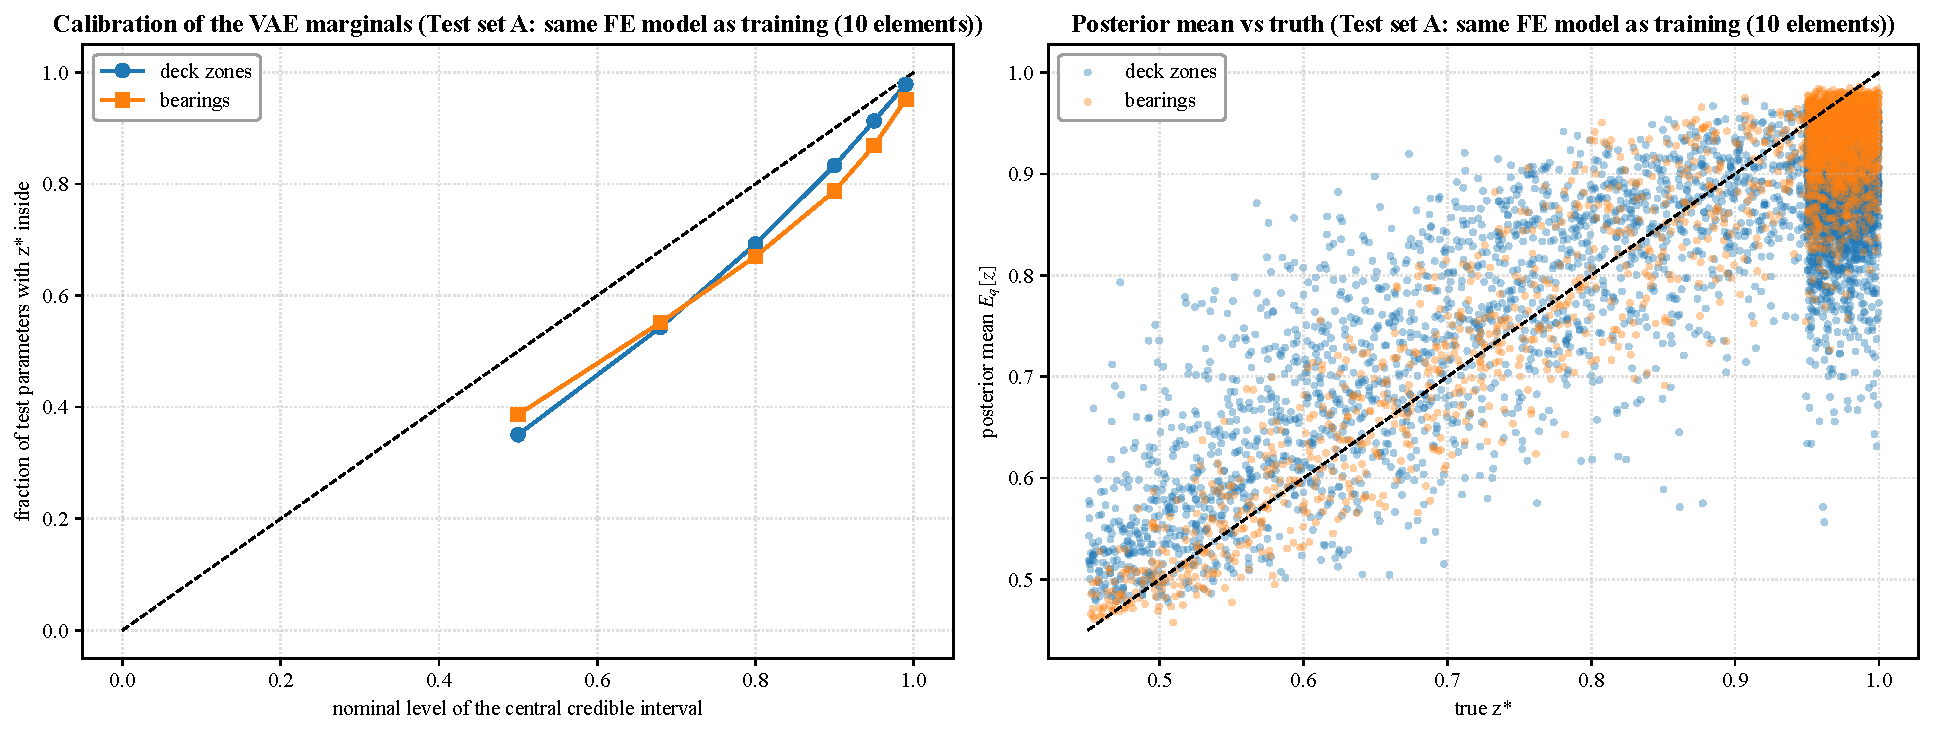
\includegraphics[width=0.9\textwidth]{figures_results/A_calibration.pdf}
\caption{Test set A, $K=3$. (a) Fraction of the test parameters whose $z^*$ lies inside the central credible interval
of the VAE marginal, against the nominal level. (b) Posterior mean against $z^*$; the band at $z^*\ge0.95$ contains
the undamaged parameters (two thirds of the test parameters).}
\label{fig:calibration}
\end{figure}

\subsection{Why the 95\% coverage is below 95\% (Editor, R1.3)}\label{sec:coverage}
Bayesian credible intervals have nominal coverage on average over the prior, not for every $z^*$. Three observations
explain most of the shortfall in Table~\ref{tab:metrics}.
\begin{enumerate}[label=(\roman*)]
\item \emph{The test set is not drawn from the prior.} The DoE places two thirds of the parameters in the top 9\% of
the prior range. As a reference, the central 95\% interval of the prior itself, $[0.464,0.986]$, has exact 95\%
coverage when $z^*$ is drawn from the prior, yet it contains only 81.1\% of the test values of $z^*$, mostly because
18.2\% of them lie above its upper limit. Coverage on the DoE test set describes the posteriors for this mix of
scenarios; it is not, by itself, a test of calibration.
\item \emph{Equal-tailed intervals exclude the region next to the bound.} For an undamaged parameter, the
equal-tailed interval leaves out the top 2.5\% of the posterior mass, which is where $z^*$ lies: $z^*$ is above the
97.5\% quantile for 9.6\% of the undamaged deck parameters and 14.2\% of the undamaged bearings, and below the 2.5\%
quantile for none. The shortfall is present at every level (Fig.~\ref{fig:calibration}a), as expected when most
$z^*$ lie in the upper tail of their marginals. Highest-density (HPD) intervals reach the bound when the density is high
there: they cover 96.6\% of the undamaged parameters and 94.6\% of all parameters (Fig.~\ref{fig:reliability}).
\item \emph{On the scenarios drawn from the prior} (120 structures, 840 parameters), the only subset on which nominal
coverage is expected and the closest analogue of the test set of the submitted manuscript, the equal-tailed coverage is
0.932 and the MACE 0.037. By type of parameter: 0.945 for the deck zones (600 parameters; binomial standard error
$\approx0.009$) and 0.900 for the bearings (240 parameters; $\approx0.014$).\footnote{The standard errors ignore the
dependence between the parameters of the same structure.} The deck zones are calibrated within the sampling error;
the bearings are not, and neither is the exact posterior (Section~\ref{sec:bearings}).
\end{enumerate}
Two cautions. First, the all-parameter HPD MACE (0.054 in A, 0.041 in B) is lower than the MACE of every group
because, with HPD intervals, some groups over-cover (the undamaged parameters and, in test set A, the deck zones) while
others under-cover (the damaged parameters and the bearings), and the deviations partly cancel; the group values
should be reported. Second, no interval
definition is right for the DoE test set as a whole: for the reason given in (ii), equal-tailed intervals under-cover
the undamaged parameters and HPD intervals over-cover them.

\begin{figure}[t]
\centering
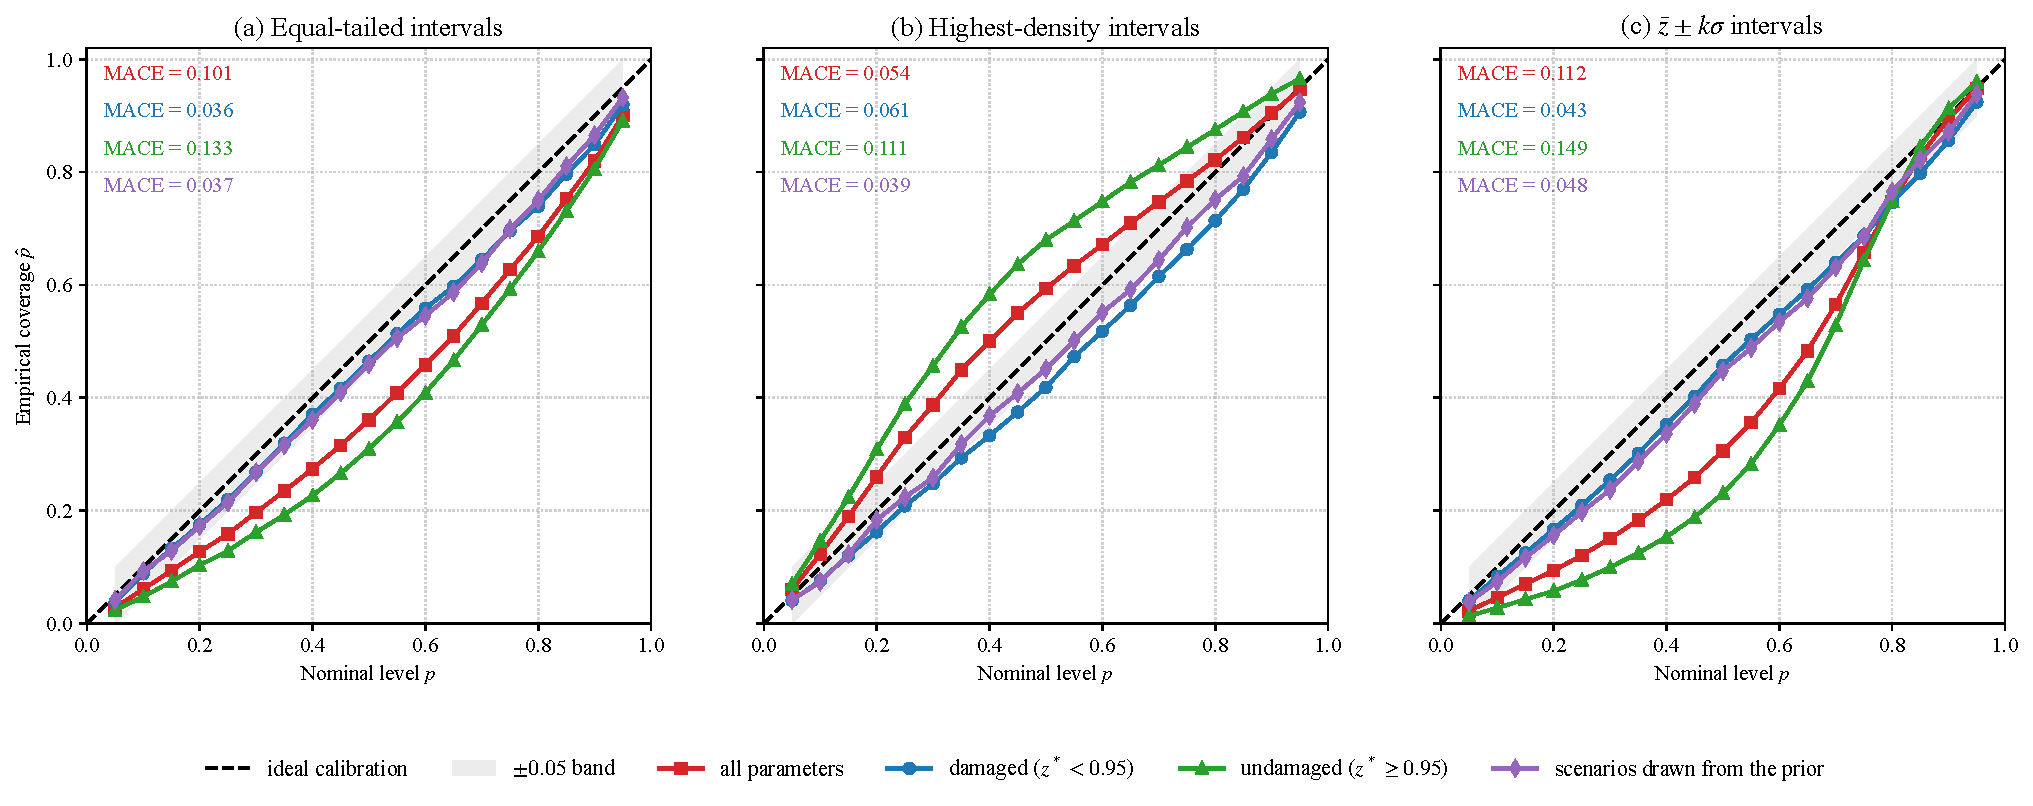
\includegraphics[width=0.85\textwidth]{figures_results/A_reliability.pdf}
\caption{Test set A, $K=3$: reliability diagrams for equal-tailed, highest-density and mean $\pm k\sigma$ intervals,
for all, damaged and undamaged parameters and for the scenarios drawn from the prior.}
\label{fig:reliability}
\end{figure}

\subsection{The bearings under-cover, and why}\label{sec:bearings}
The bearings have the narrowest posteriors (mean width of the 95\% interval 0.149, against 0.259 for the deck zones)
and the lowest coverage in every scenario category: 0.85--0.90 in test set A, against 0.89--0.95 for the deck zones
(overall 0.869 and 0.913). Most misses are undamaged bearings whose $z^*$ lies above the interval (14.2\%), i.e.\ the
posterior says that the pad is softer than it is; this is also why the bearings have the highest false-alarm rates
(Table~\ref{tab:param}). On the benchmarks, 4 of the 22 bearing parameters lie outside the exact 95\% interval,
against 5 of the 55 deck parameters (Table~\ref{tab:bench}).

\paragraph{The exact posterior under-covers the bearings too.} We computed the exact posteriors of the 120 structures
drawn from the prior (script \texttt{prior\_scenarios\_coverage.py}; Table~\ref{tab:prior_cov},
Fig.~\ref{fig:prior_cov}). In test set A the exact posterior covers the deck zones at the nominal rate (0.957) but not
the bearings (0.904, 2.2 standard errors below 0.95), and the PIT of the bearings is U-shaped: $z^*$ falls in both
tails too often (5.4\% below the 2.5\% quantile, 4.2\% above the 97.5\% quantile), the signature of posteriors that are
too narrow. The VAE has the same bearing coverage (0.900; exact minus VAE: $0.004\pm0.007$). The under-coverage of the
bearings therefore comes from the likelihood, not from the VAE. For the deck zones the VAE loses about one point with
respect to the exact posterior ($0.012\pm0.005$).

\begin{table}[t]
\centering\footnotesize
\caption{Coverage of the central 95\% interval on the 120 test structures drawn from the prior: exact (SMC) and VAE
($K=3$) posteriors, $\pm$ bootstrap standard error over structures; MACE over 19 levels in parentheses.}
\label{tab:prior_cov}
\setlength{\tabcolsep}{4pt}
\begin{tabular}{l cc cc}
\toprule
 & \multicolumn{2}{c}{Test set A} & \multicolumn{2}{c}{Test set B} \\
\cmidrule(lr){2-3}\cmidrule(lr){4-5}
 & Exact & VAE & Exact & VAE \\
\midrule
Deck zones (600)  & $0.957\pm0.008$ (0.015) & $0.945\pm0.010$ (0.022) & $0.905\pm0.012$ (0.054) & $0.903\pm0.013$ (0.061) \\
Bearings (240)    & $0.904\pm0.021$ (0.068) & $0.900\pm0.020$ (0.074) & $0.842\pm0.025$ (0.094) & $0.825\pm0.025$ (0.106) \\
All (840)         & $0.942\pm0.009$ (0.029) & $0.932\pm0.010$ (0.037) & $0.887\pm0.012$ (0.065) & $0.881\pm0.012$ (0.074) \\
\bottomrule
\end{tabular}
\end{table}

\begin{figure}[t]
\centering
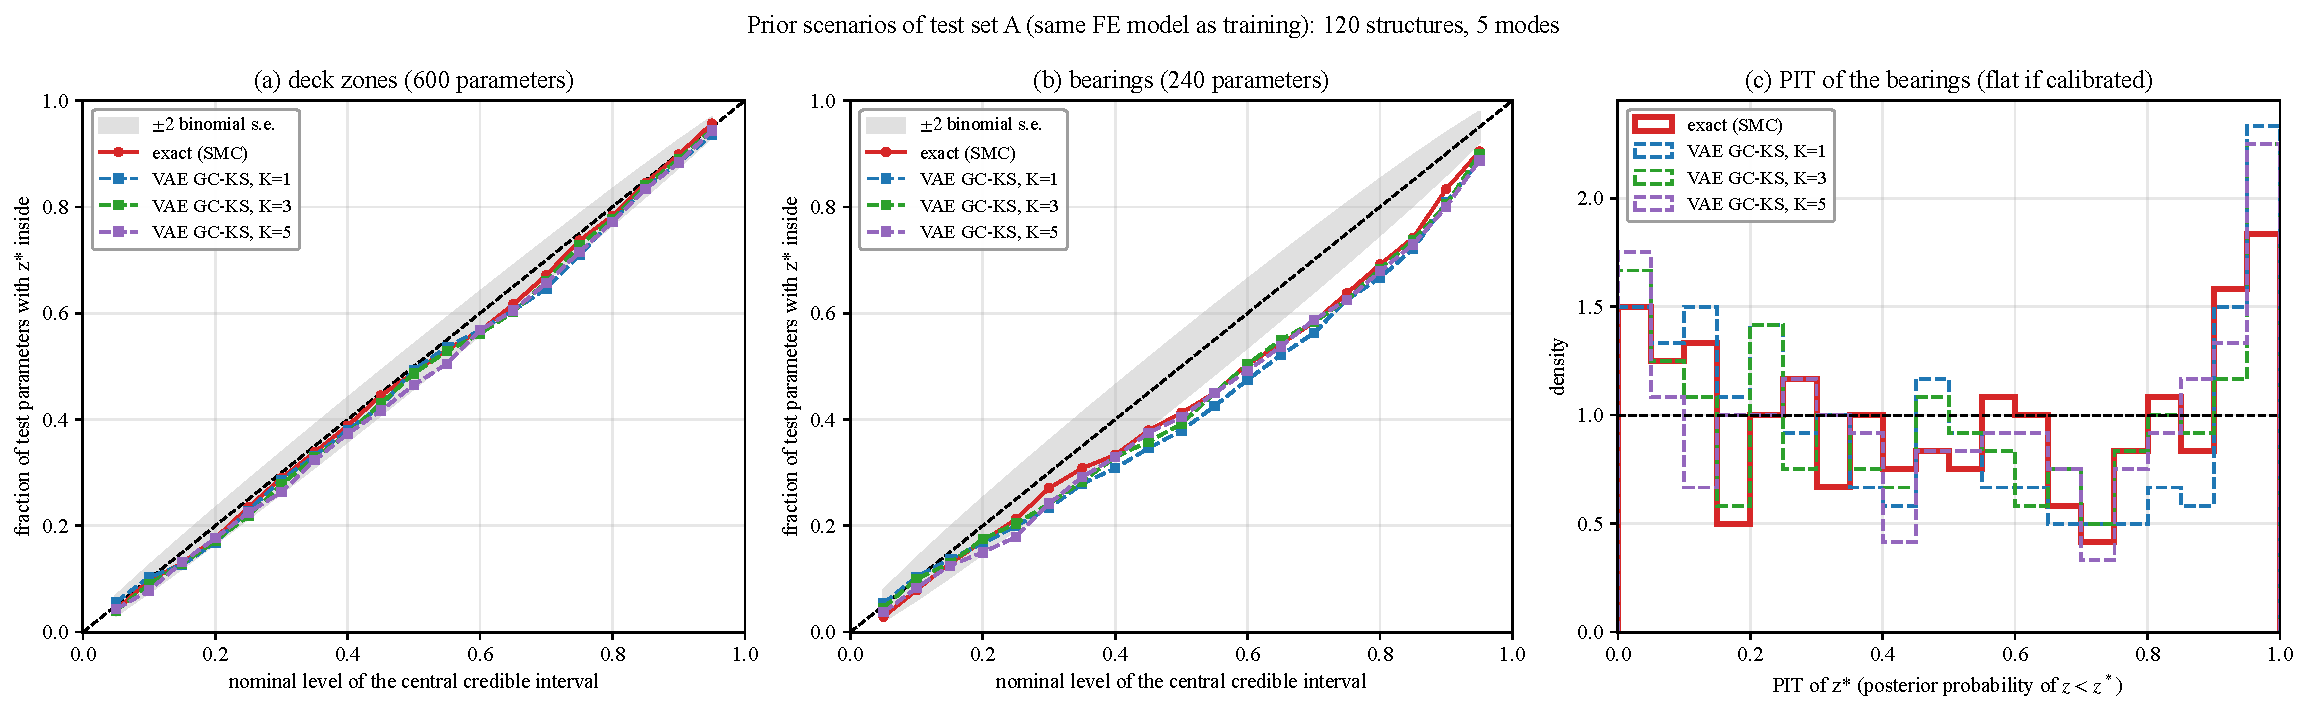
\includegraphics[width=\textwidth]{figures_results/A_prior_scenarios_coverage.pdf}
\caption{Prior scenarios of test set A (120 structures): coverage of the central intervals against their level for
the deck zones (a) and the bearings (b), exact (SMC) and VAE posteriors with $K=1,3,5$; (c) PIT of the bearings (flat if
calibrated; U-shaped if the posteriors are too narrow).}
\label{fig:prior_cov}
\end{figure}

\paragraph{Cause: the mode-shape term assumes isotropic errors.} The likelihood scores the shape misfit of mode $m$ as an
isotropic Gaussian in the four directions orthogonal to the predicted shape, with one variance $\sigma_{v,m}^2$
calibrated on average. On average the shape terms are right (training generator: ratios 0.99--1.01), which is why the
calibration check did not reveal the problem; their structure is not (Table~\ref{tab:shape_error}, computed on the
training data against noise-only simulations):
\begin{itemize}
\item In modes 4 and 5 the as-built error is concentrated in one direction: the largest eigenvalue of the residual
covariance holds 44\% and 42\% of the variance, against 26\% for the measurement noise alone (25\% if isotropic). This
error comes almost entirely from the mass field (error budget: mean $1-\mathrm{MAC}$ of 0.0018 and 0.0033 in modes 4
and 5, against at most $5\times10^{-6}$ for the stiffness scatter).
\item That direction is close to the directions in which the bearings change those shapes: along them, the actual
misfit variance is 1.6--1.7 times $\sigma_{v,m}^2$.
\item The bearings draw 68\% of their mode-shape information from modes 4 and 5; the deck zones draw theirs mostly
from directions where the ratio is 0.8--1.2.
\end{itemize}
The likelihood therefore over-weights the mode-shape evidence about the bearings, and their posteriors are too narrow.
Two consistent symptoms: the shape terms of modes 4 and 5 have heavier tails than the isotropic model (1.7\% and 1.4\%
of the training structures above its 99\% quantile, against 1.0\%), and in the prior scenarios whose bearings the exact
posterior misses, the shape terms of modes 3--5 at $z^*$ are 1.4--1.8 times their expected value, against 0.8--1.1 for
the others (part of this contrast is expected by selection). The covariances were computed for the healthy structures;
the directions change with damage. A candidate fix is a full covariance of the shape residual of each mode, calibrated
like the frequency covariance. We have not tested it: exact posteriors of the prior scenarios under that likelihood
would show in a few minutes whether it restores the coverage of the bearings, before any retraining.

\begin{table}[t]
\centering\footnotesize
\setlength{\tabcolsep}{4pt}
\caption{Structure of the mode-shape error (script \texttt{shape\_error\_structure.py}; 14,000 training structures,
covariances from the 1,400 healthy ones).
Share: largest eigenvalue of the covariance of the shape residual orthogonal to the predicted shape (isotropic: 0.25).
Ratio: residual variance along the direction in which the parameter changes the shape, divided by the variance
$\sigma_{v,m}^2$ assumed by the likelihood (1: correct weight; $>1$: the likelihood over-weights that evidence). Last
column: share of the mode-shape information about a bearing carried by each mode.}
\label{tab:shape_error}
\begin{tabular}{c cc cccc c}
\toprule
 & \multicolumn{2}{c}{Largest-eigenvalue share} & \multicolumn{4}{c}{Variance ratio along the direction of} & Bearing \\
\cmidrule(lr){2-3}\cmidrule(lr){4-7}
Mode & as built & noise only & $z_1$, $z_5$ & $z_2$, $z_4$ & $z_3$ & bearings & information \\
\midrule
1 & 0.27 & 0.27 & 1.00--1.03 & 1.02--1.06 & 0.94 & 0.97--1.02 & 0.00 \\
2 & 0.29 & 0.27 & 0.96--0.98 & 0.92--1.04 & 0.90 & 0.93--0.95 & 0.07 \\
3 & 0.31 & 0.26 & 1.18--1.19 & 1.02--1.05 & 0.90 & 1.07--1.09 & 0.24 \\
4 & 0.44 & 0.26 & 1.60       & 0.91--0.92 & 0.81 & 1.67--1.68 & 0.40 \\
5 & 0.42 & 0.26 & 1.13--1.17 & 1.34--1.39 & 0.97 & 1.56--1.61 & 0.28 \\
\bottomrule
\end{tabular}
\end{table}

% =============================================================================
\section{What sets the width of the posteriors}\label{sec:width}

\subsection{Physics}
The posterior widths follow the energy shares of Table~\ref{tab:param}: the end zones have the widest posteriors
(mean std 0.084 undamaged, 0.097--0.100 damaged), the inner zones intermediate ones (0.051--0.071) and the bearings
the narrowest (0.037--0.042). The exact posteriors show the same ordering for the deck: for P0 the exact std is 0.084
($z_1$) and 0.109 ($z_5$), against 0.035--0.042 for the inner zones. We have not separated the contributions of the
frequencies and of the mode shapes, so we cannot say how much of the narrowness of the bearings comes from each.
Undamaged parameters have slightly narrower posteriors than damaged ones, consistent with the truncation of their
posteriors at $z=1$.

Observations of the same damage state can give quite different posteriors, by amounts comparable to these widths.
P1 and P8 have the same damage ($z_1^*=0.56$) but different as-built structures and noise draws; the exact posterior of
$z_1$ is $0.541\pm0.072$ for P1 and $0.733\pm0.109$ for P8.

\subsection{Measurement noise and modelling error (R1.2, R3.1)}
All observations come from as-built structures whose mass and stiffness deviations the decoder ignores. Their effect
is included in the likelihood, which was calibrated by simulation on the training generator. For the logarithm of the
frequencies, the standard deviation is 2.5\% from the noise and 0.90--1.08\% from the modelling error (total
2.66--2.72\%); for the vertical shapes, $\sigma_v=0.028$--$0.044$, of which the noise alone gives 0.027--0.033, while
the modelling error grows with the mode (0.001 in mode 1, 0.029 in mode 5). The modelling error thus widens the
likelihood by 6--9\% for the frequencies and by 0--33\% for the mode shapes (most in mode 5), and the posteriors
include this widening. Measurement noise remains the dominant source for the frequencies. On test set A the data
terms at $z^*$ match their expected values, and the deck zones are calibrated on the prior scenarios
(Section~\ref{sec:coverage}): the unmodelled mass and stiffness deviations do not make the deck posteriors
over-confident. They do make the bearing posteriors over-confident, through the mode shapes of modes 4 and 5, whose
as-built errors are not isotropic as the likelihood assumes (Section~\ref{sec:bearings}). We did not train a model with a noise-only
likelihood, so we cannot yet say how much wider the posteriors are because of the modelling error. Exact posteriors of
the benchmarks under both likelihoods would answer this at a small cost.

\subsection{Detection limits and false alarms (R1.6)}
We declare a parameter damaged when the upper limit of its 95\% equal-tailed interval is below 0.95, i.e.\ when the
posterior probability of $z_d<0.95$ exceeds 0.975. By severity (Table~\ref{tab:param}):
\begin{itemize}
\item inner zones: severe damage ($z^*<0.60$) detected in 97--100\% of the cases, moderate damage (0.60--0.75) in
72--81\%, mild damage (0.75--0.90) in 15--27\%;
\item end zones: 76--83\%, 35--39\% and 7--10\%;
\item bearings: 100\%, 98\% and 51--52\%;
\item damage in $[0.90,0.95)$: 2.6\% (deck) and 13.2\% (bearings).
\end{itemize}
These limits follow from the sensitivities of Section~\ref{sec:case}: mild damage changes the data by less than the
noise, and by even less in the end zones. They are limits of the information in the data, not of the VAE. The exact
posteriors agree: in P10 ($z_4^*=0.90$) the exact posterior of $z_4$ is $0.936\pm0.050$, indistinguishable from a
healthy zone, while in P3 ($z_2^*=0.78$) it is $0.755\pm0.072$.

The false-alarm rate per parameter is 0.4--1.1\% for the deck zones and 2.8--3.7\% for the bearings. Since seven
parameters are tested per structure, 11.7\% of the 120 healthy structures have at least one parameter declared
damaged (in both test sets). This is the figure that matters for an operator. A stricter rule would lower it at the
cost of detection; we have not computed that trade-off.

% =============================================================================
\section{Dependence between parameters (copula)}\label{sec:copula}
Figure~\ref{fig:copula} summarizes the copula correlations of the VAE posteriors on test set A. Adjacent deck zones
are negatively correlated (median $-0.08$ when both are undamaged, $-0.15$ with one damaged, $-0.20$ with both
damaged), and so are an end zone and its adjacent bearing ($-0.22$); the two bearings are positively correlated
($+0.27$), and opposite zones are practically uncorrelated ($+0.02$).

\paragraph{Meaning.} A negative correlation expresses a trade-off: the stiffness losses of the two parameters change
the data in similar ways, so the data constrain a combination of them better than each one separately. A softer end
zone and a softer adjacent pad both lower the frequencies of the modes in which they store energy, and along the
direction in which one is stiffer and the other softer the data change little. The positive correlation of the
bearings means that their sum is less determined than their difference: at the healthy state, the linearized
(Laplace) posterior has a standard deviation of 0.090 for $(\zb{L}+\zb{R})/\sqrt2$ and of 0.058 for
$(\zb{L}-\zb{R})/\sqrt2$.

\paragraph{Evidence that the correlations are physical.} (a) The exact posteriors of the benchmarks have the same
signs: $z_1$--$\zb{L}$ between $-0.10$ and $-0.43$, $\zb{L}$--$\zb{R}$ between $+0.11$ and $+0.35$, adjacent zones
negative, opposite zones close to zero. (b) The linearized posterior at the healthy state gives the same signs
($z_1$--$\zb{L}$ $-0.51$, $\zb{L}$--$\zb{R}$ $+0.41$, $z_2$--$z_3$ $-0.37$, $z_1$--$z_2$ $-0.20$) with larger
magnitudes; it ignores the bounds, whose truncation of the healthy parameters reduces the correlations of the exact
posterior. (c) The VAE reproduces the exact correlation matrices with a Frobenius error of 0.13--0.26, i.e.\ about
0.02--0.04 per entry (Section~\ref{sec:exact}).

\paragraph{Consequence for individual scenarios.} The errors of both the exact and the VAE posteriors with respect to
$z^*$ often lie along these trade-off directions. In P5 ($z_1^*=0.60$, $\zb{L}^*=0.58$; Fig.~\ref{fig:marginals}a)
the posteriors assign the loss mostly to the pad ($\zb{L}$: $0.495\pm0.027$) and too little to zone 1
($0.772\pm0.105$); the exact correlation of $z_1$ and $\zb{L}$ in P5 is $-0.33$. P7 shows the opposite shift
($z_1$: 0.538 for $z^*=0.62$; $\zb{L}$: 0.809 for $z^*=0.68$). In P6, the damaged zone 2 is under-estimated (0.618
for $z^*=0.54$) while its healthy neighbours appear damaged ($z_1$: 0.789; $z_3$: 0.734), consistent with the negative
correlation of adjacent zones.

\paragraph{Strength of the dependence and effect on the joint density.} The dependence is modest: the total
correlation of the copula, $-\tfrac12\log\det\mathbf R$, is 0.30 nats on average (0.15 for the healthy structures,
0.54 for the prior scenarios). On test set A, the joint log density at $z^*$ (copula included) is lower than the sum
of the marginal log densities: the copula term $\log c(\mathbf u^*)$ averages $-0.48$ nats per structure (joint ALL
per parameter 0.976 against 1.044 for the marginals). It is negative where many parameters are undamaged (healthy
structures $-1.10$, one damaged parameter $-0.75$, two $-0.51$) and close to zero otherwise (three $-0.12$, four or
five $+0.04$, prior scenarios $-0.03$). The negative values have a simple origin: the $z^*$ of an undamaged parameter
lies in the upper tail of its marginal, so its normal score $\Phi^{-1}(F_d(z^*))$ is large and positive, and for two
such parameters with a negative copula correlation $\log c$ is negative (for $\rho=-0.15$ and two scores equal to 2,
$\log c\approx-0.7$). It is the same selection effect as in Section~\ref{sec:coverage}. On the prior scenarios, if
$z^*$ were distributed as the VAE posterior, the expected value of the copula term would be the total correlation,
$+0.54$ nats; we obtain $-0.03$, and we do not know why. The marginal mis-calibration of the bearings changes the
normal scores and may contribute, but we have not separated the effects. In short, the copula reproduces the
trade-offs of the exact posterior, but on these test sets it does not increase the density at $z^*$.

\begin{figure}[t]
\centering
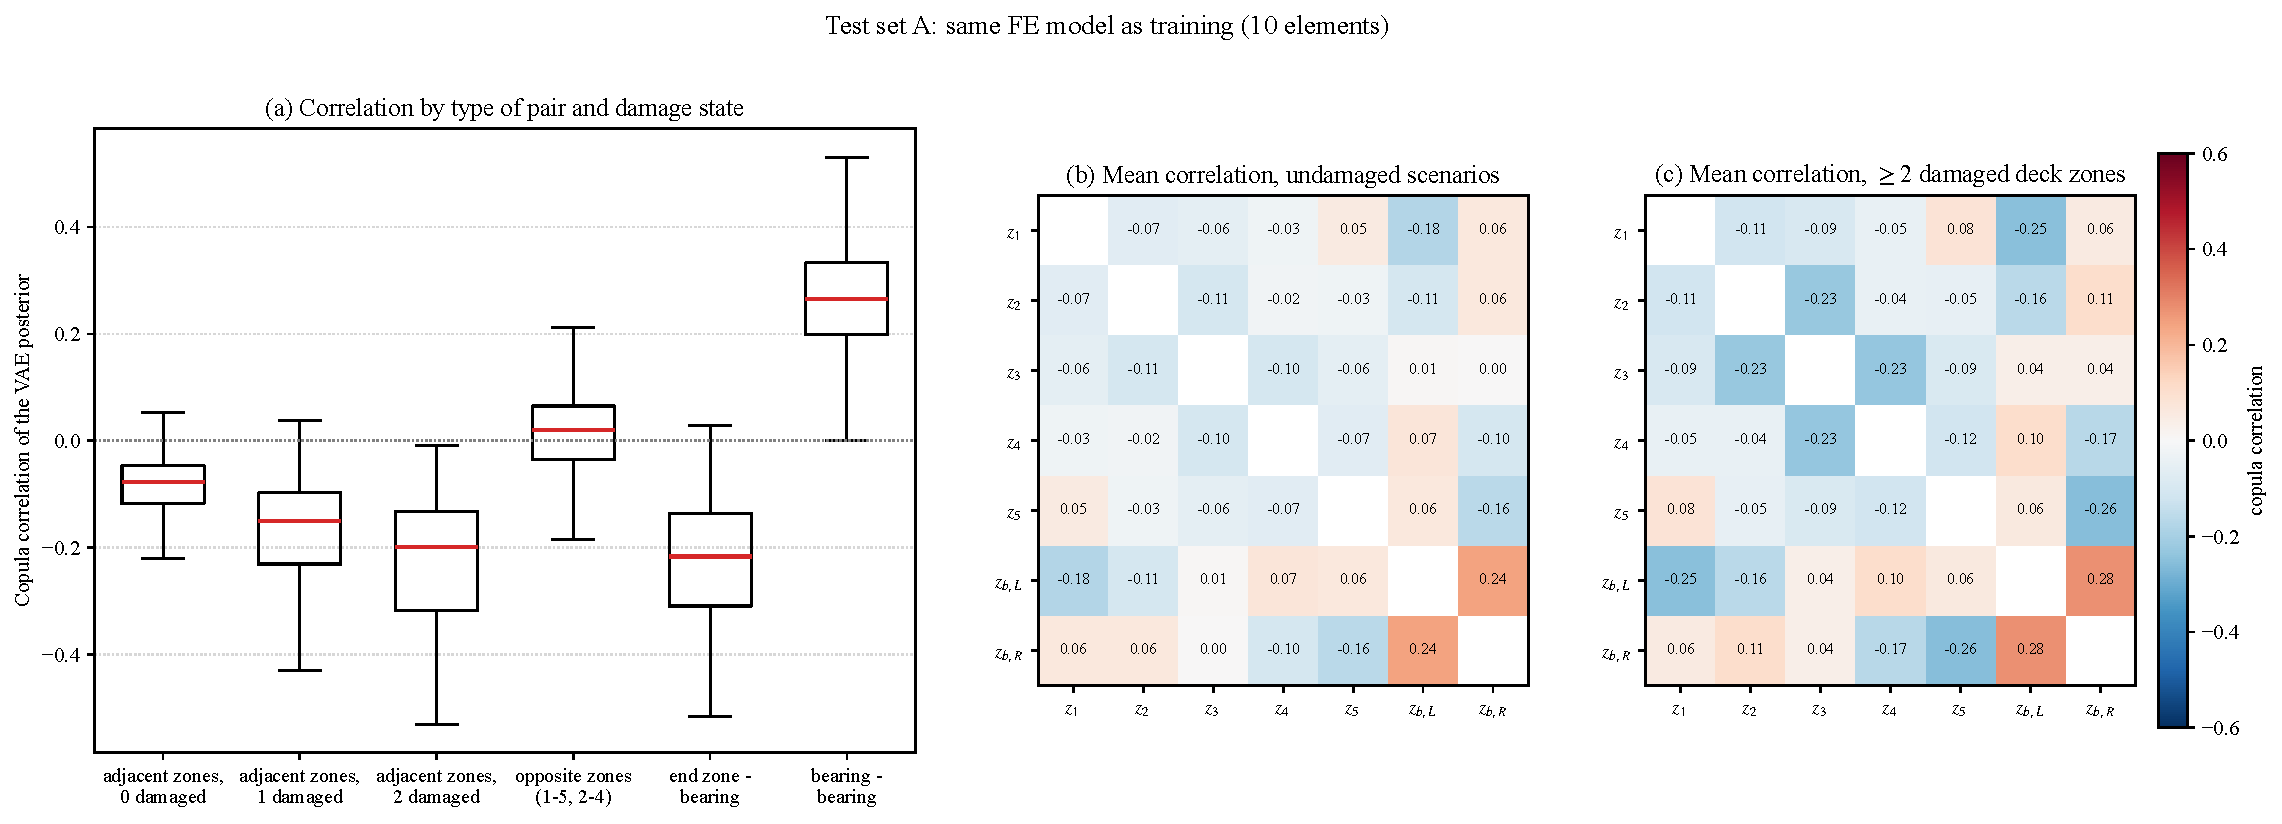
\includegraphics[width=\textwidth]{figures_results/A_copula_correlations.pdf}
\caption{Copula correlations of the VAE posteriors, test set A, $K=3$: (a) distribution by type of pair and damage
state; (b) mean correlation matrix for undamaged scenarios; (c) mean correlation matrix for scenarios with at least
two damaged deck zones.}
\label{fig:copula}
\end{figure}

% =============================================================================
\section{VAE versus exact posteriors}\label{sec:exact}
On the 11 benchmarks of test set A, the means of the VAE and exact marginals differ by 0.003 on average (at most
0.010), the ratio of their standard deviations is 0.99 on average (0.92--1.07 per marginal), the 1-Wasserstein
distance is 0.003 and the Frobenius error of the correlation matrix 0.13--0.26. On test set B: 0.004 (at most
0.015), 0.99 (0.90--1.10), 0.004 and 0.13--0.29. The VAE and exact marginals of Fig.~\ref{fig:marginals} overlap. All
the marginals in this figure, and in P7 of test set A, which we also inspected, are unimodal; many are piled against
a bound.

Every parameter outside the exact 95\% interval is also outside the VAE interval (Table~\ref{tab:bench}). The VAE
misses two more parameters in test set A (both in P0) and four more in test set B; since means and standard
deviations agree to within 0.015 and 10\%, $z^*$ must lie close to the interval limits in those cases. The errors with
respect to the truth that remain in the benchmarks, such as the healthy zones that appear damaged in P1 ($z_2$:
0.807, $z_3$: 0.846), P6 and P10, or the zone--bearing mix-up of P5, are present in the exact posteriors. In test set
A an observation differs from the nominal model at $z^*$ only through the noise and the as-built deviations of that
structure, so these errors come from the information content of each observation, not from the amortized inference.

Beyond the benchmarks, the 120 prior scenarios of Section~\ref{sec:bearings} give a larger comparison. In test set A,
the means differ by 0.005 on average (at most 0.041), the ratio of standard deviations is 0.99 on average (0.82--1.14),
the 1-Wasserstein distance is 0.006 and the Frobenius error of the correlation matrix 0.12--0.44 (mean 0.25); in test
set B: 0.007 (0.052), 0.99 (0.62--1.32), 0.007 and 0.12--0.72 (0.28). The agreement is weaker than on the
benchmarks (mean differences and $W_1$ about twice as large, wider extremes), but the coverage of the VAE stays within
about one point of the exact one (Table~\ref{tab:prior_cov}).
On the 2,400 validation observations the importance-weighted diagnostics agree: the lower bound of $\mathrm{KL}(q\|p)$
is 0.065 nats on average, and $\hat k$ is below 0.5 for 89\% and below 0.7 for 99\% of the observations
(Section~\ref{sec:baselines}).

\begin{table}[t]
\centering\footnotesize
\setlength{\tabcolsep}{4pt}
\caption{Benchmarks ($K=3$): parameters whose $z^*$ lies outside the central 95\% interval of the exact (SMC)
posterior, and parameters outside the VAE interval only. In parentheses ($z^*$; exact posterior mean $\pm$ std),
test set A.}
\label{tab:bench}
\begin{tabular}{l l l l l l}
\toprule
 & Scenario & \multicolumn{2}{c}{Outside the exact 95\% interval} & \multicolumn{2}{c}{Outside for the VAE only} \\
\cmidrule(lr){3-4}\cmidrule(lr){5-6}
 & & Test set A & B & A & B \\
\midrule
P0  & healthy                         & --- & --- & $z_5$, $\zb{L}$ & $z_5$, $\zb{L}$ \\
P1  & $z_1=0.56$                      & $z_2$ (0.98; $0.81\pm0.08$), $z_3$ (0.99; $0.85\pm0.08$) & $z_2$, $z_3$ & --- & --- \\
P2  & $z_3=0.65$                      & --- & --- & --- & --- \\
P3  & $z_2=0.78$                      & $\zb{L}$ (0.98; $0.87\pm0.05$) & $\zb{L}$ & --- & --- \\
P4  & $\zb{L}=0.55$                   & --- & --- & --- & --- \\
P5  & $z_1=0.60$, $\zb{L}=0.58$       & $\zb{L}$ (0.58; $0.50\pm0.03$) & --- & --- & $\zb{L}$ \\
P6  & $z_2$, $z_4$, $\zb{R}$ damaged  & $z_3$ (0.98; $0.73\pm0.10$) & --- & --- & $z_3$ \\
P7  & five damaged                    & $\zb{L}$ (0.68; $0.81\pm0.05$) & $\zb{L}$ & --- & --- \\
P8  & $z_1=0.56$, other draw          & $z_3$ (0.99; $0.83\pm0.08$) & $z_1$, $z_3$ & --- & --- \\
P9  & $z_2$, $\zb{L}$ damaged         & --- & --- & --- & --- \\
P10 & $z_4=0.90$                      & $z_1$ (0.99; $0.74\pm0.11$), $\zb{R}$ (0.98; $0.86\pm0.05$) & $z_1$, $\zb{R}$ & --- & --- \\
\midrule
\multicolumn{2}{l}{$z^*$ inside the 95\% interval} & exact: 68/77 & 69/77 & VAE: 66/77 & 65/77 \\
\bottomrule
\end{tabular}
\end{table}

% =============================================================================
\section{Test set B: refined model and localized damage (R1.1, R2.3)}\label{sec:testB}
\paragraph{What changes.} Refining the mesh alone (50 elements, nominal structure) changes $\log f$ by at most 0.13\%
(mode 5): the 10-element model is converged for the first five modes. What makes test set B different is the localized
damage, which adds a standard deviation of 0.74--1.58\% to $\log f$ depending on the mode. The total modelling error
grows from 0.91--1.09\% (test set A) to 1.20--1.82\% (test set B). The data terms at $z^*$ exceed their expected
values by 15\% for the frequencies and by 0--32\% for the mode shapes (ratios 1.00, 1.14, 1.27, 1.31 and 1.32 for
modes 1--5): the likelihood is too narrow for test set B, more so for the higher modes.

\paragraph{Effect.} The posteriors keep their width (mean width of the 95\% interval 0.223 against 0.228), but the data
are more surprising (Table~\ref{tab:metrics}): ALL drops from 1.044 to 0.965, the equal-tailed coverage from 0.900 to
0.883 (HPD: 0.946 to 0.923), the MACE of the damaged parameters rises from 0.037 to 0.063, the coverage of the prior
scenarios drops from 0.932 to 0.881 and that of the bearings from 0.869 to 0.840, and the false alarms rise from 1.5\%
to 2.3\% of the undamaged parameters; the detection rate barely changes (64.2\% and 63.1\% of the parameters with
$z^*<0.90$). The degradation is moderate and has the direction expected under an unmodelled discrepancy
(over-confidence). The VAE still matches the exact posteriors (Section~\ref{sec:exact}), so the degradation comes from
the data, not from a poor generalization of the encoder. On the prior scenarios the exact posterior itself covers
0.905 (deck zones) and 0.842 (bearings), and the VAE 0.903 and 0.825 (Table~\ref{tab:prior_cov}). The misses of the
bearings are now mostly on one side ($z^*$ above the interval in 10.8\% of the cases, below in 5.0\%): the posterior
makes the pads too soft. We have not checked whether this comes from localized damage of the end zones being
attributed to the pads, as in P5.

\paragraph{The zone parameter is an energy-weighted equivalent stiffness.} The label $z^*$ of a zone with localized
damage is the harmonic mean of the stiffness over the zone, but the modal data weight a stiffness loss by the local
strain energy (Section~\ref{sec:case}), which is small next to the supports in every mode. The exact posteriors of three
benchmarks, with the same structure and noise in both test sets, show the consequence (zone 1 spans $x=0$--2~m):
\begin{itemize}
\item P5: damage over $x=1.2$--2.0~m (local factor 0.38), the inner end of zone 1; posterior mean of $z_1$: 0.772 (A),
0.532 (B), for $z^*=0.60$ (Fig.~\ref{fig:marginals}a,b);
\item P8: damage over $x=0$--1.6~m (factor 0.50), next to the support: 0.733 (A), 0.797 (B), for $z^*=0.56$, which in
test set B lies outside the exact 95\% interval (Fig.~\ref{fig:marginals}c);
\item P1: damage over $x=0.2$--2.0~m (factor 0.53), almost uniform: 0.541 (A), 0.524 (B), for $z^*=0.56$.
\end{itemize}
The test-set statistics agree: severe damage ($z^*<0.60$) in the end zones is detected in 65\% of the cases in test set
B against 76--83\% in test set A, whereas for the inner zones and the bearings it stays at 97--100\% in both
(Table~\ref{tab:param}). Damage concentrated next to a support is therefore hard to identify with this parametrization
and these data.

\begin{figure}[t]
\centering
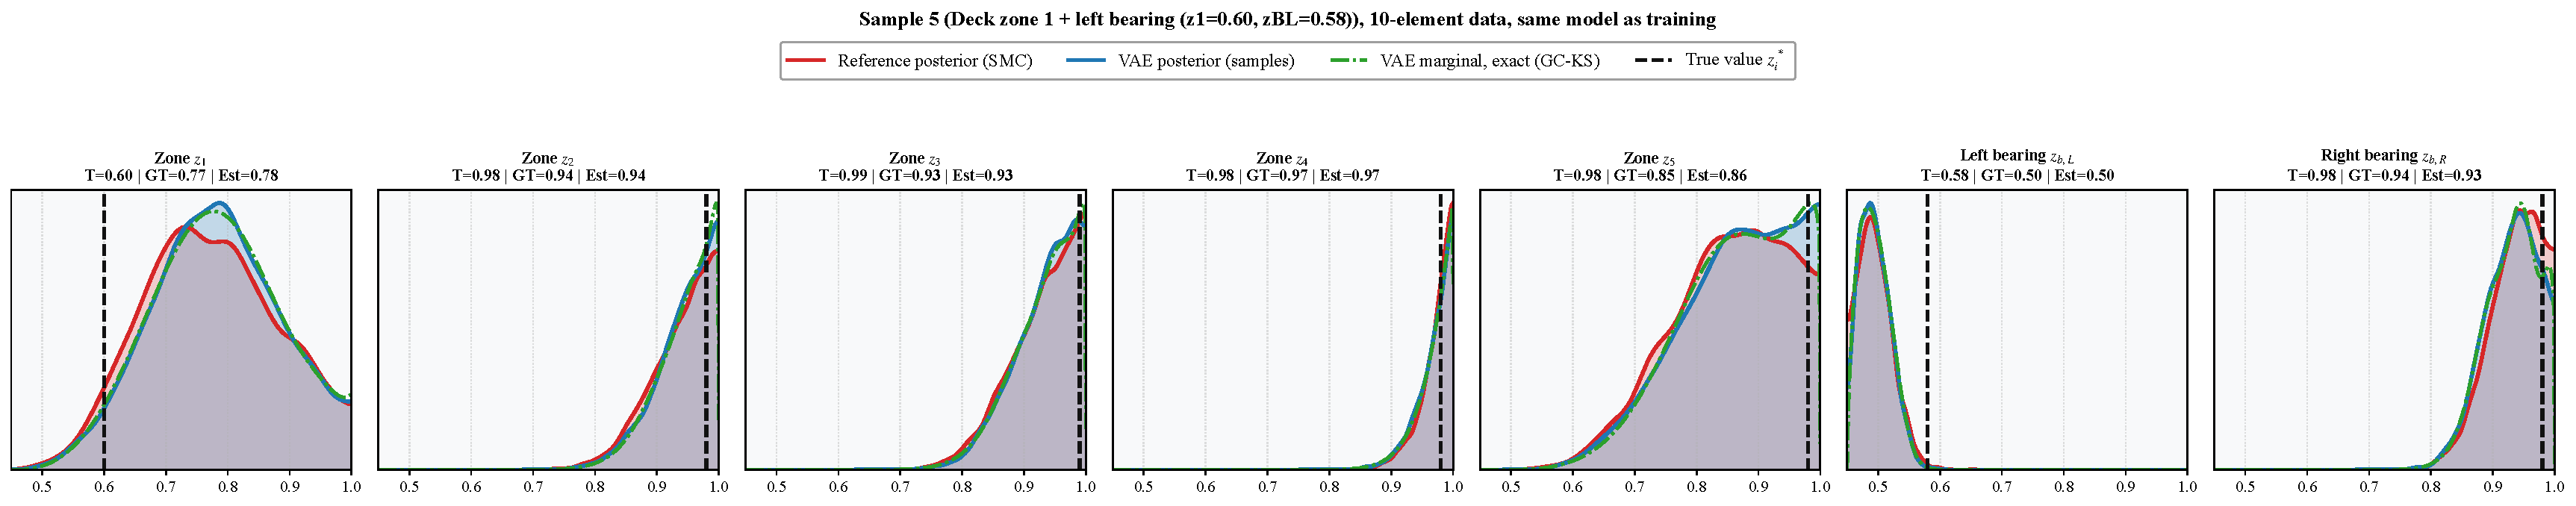
\includegraphics[width=\textwidth]{figures_results/A_P5_1D.pdf}\\[2pt]
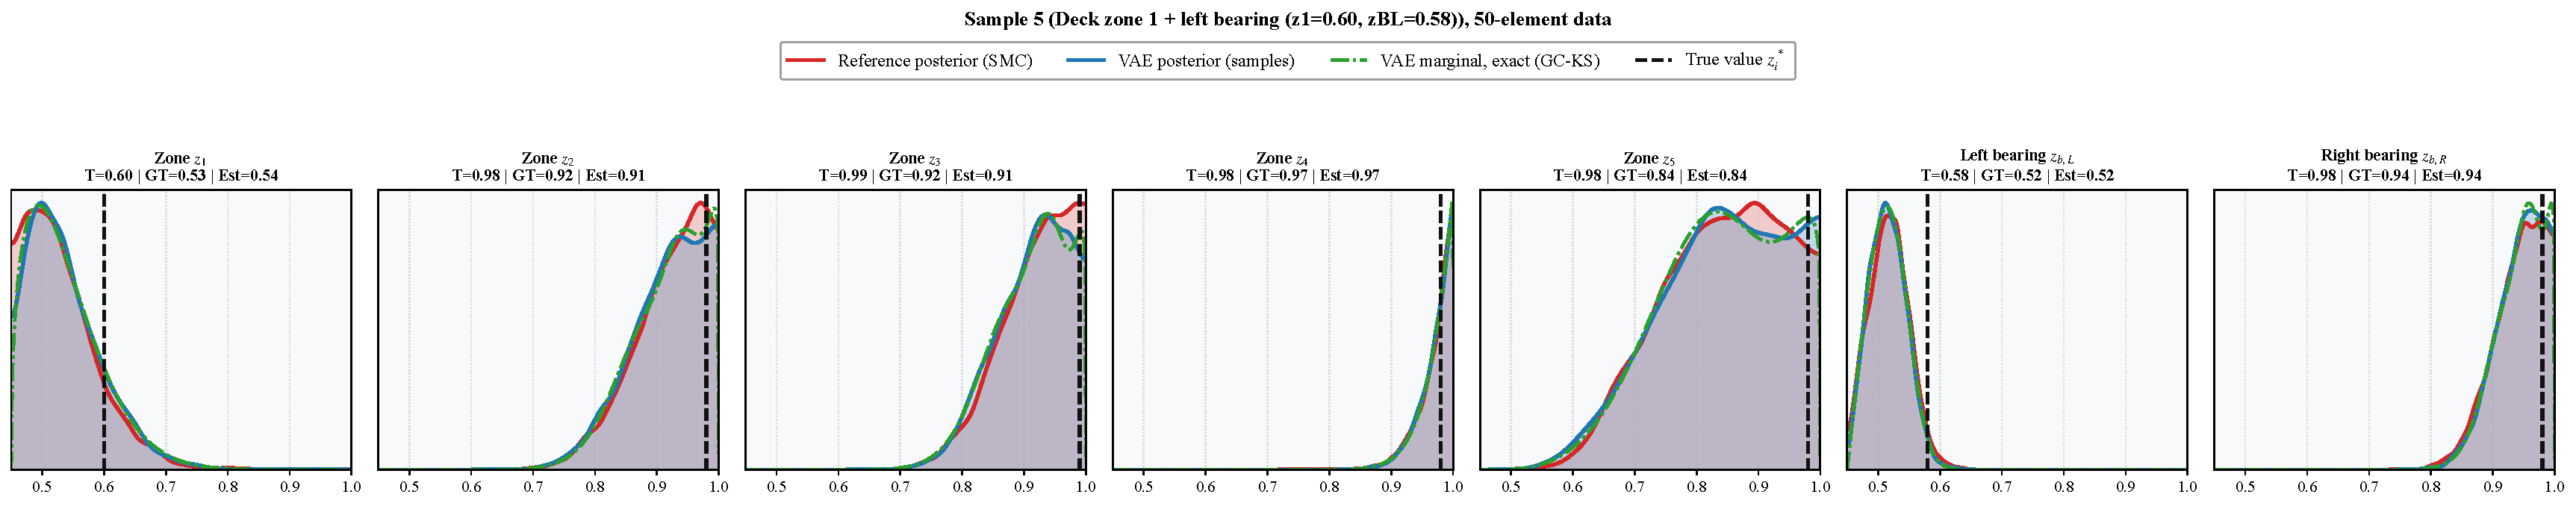
\includegraphics[width=\textwidth]{figures_results/B_P5_1D.pdf}\\[2pt]
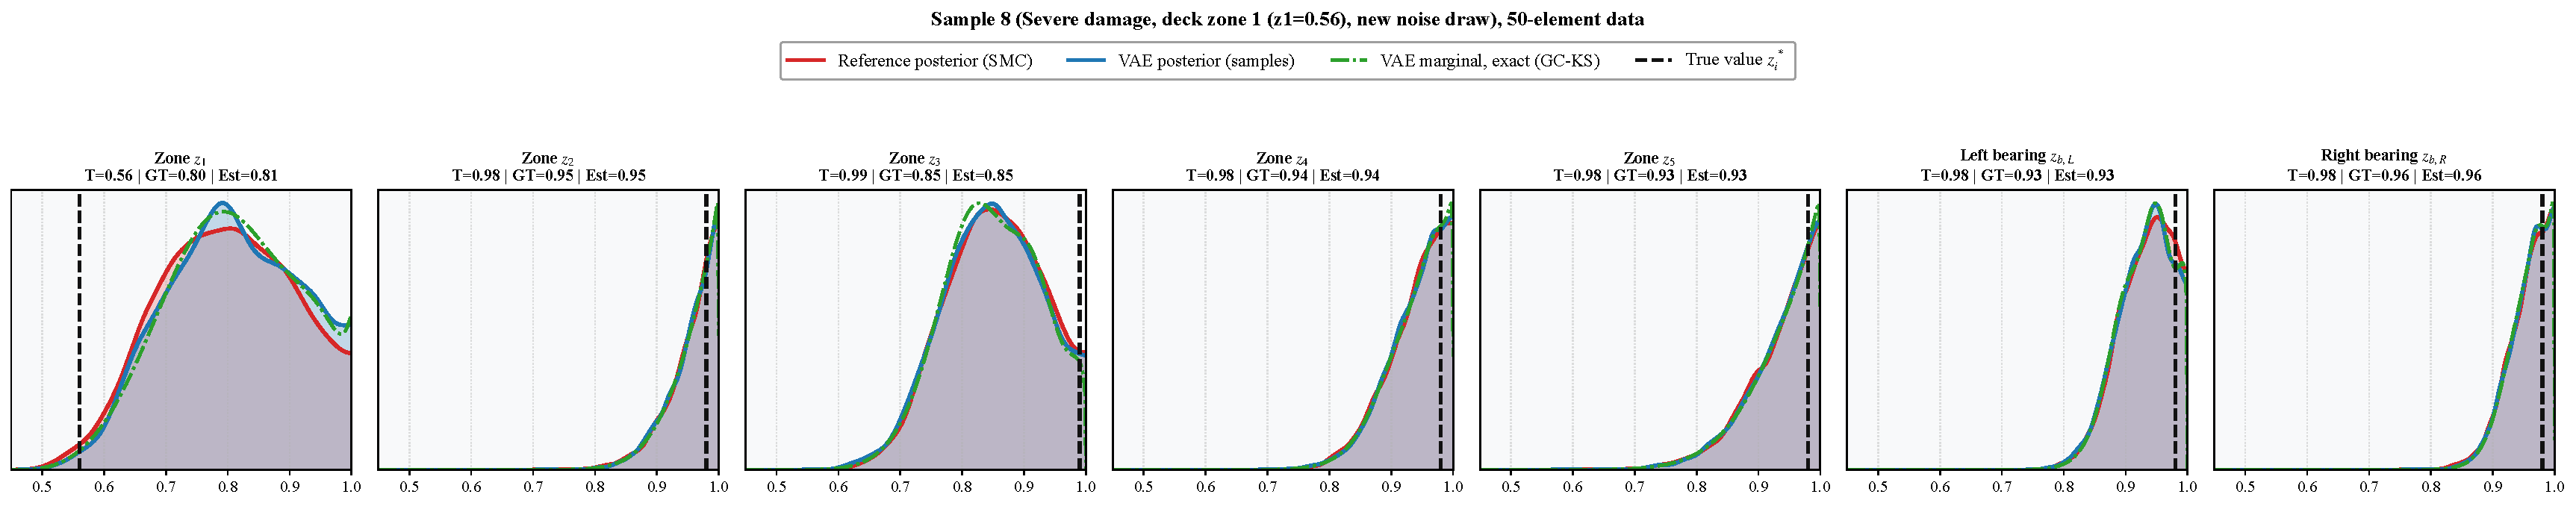
\includegraphics[width=\textwidth]{figures_results/B_P8_1D.pdf}
\caption{Marginals of the exact (SMC) and VAE posteriors ($K=3$); dashed lines: $z^*$. (a) P5, test set A; (b) P5,
test set B (damage of zone 1 concentrated in $x=1.2$--2.0~m); (c) P8, test set B (damage of zone 1 concentrated in
$x=0$--1.6~m).}
\label{fig:marginals}
\end{figure}

% =============================================================================
\section{Number of Kumaraswamy components}\label{sec:K}
\begin{table}[t]
\centering\footnotesize
\caption{GC--KS with $K=1,3,5$ components (one seed).}
\label{tab:K}
\begin{tabular}{l ccc}
\toprule
 & $K=1$ & $K=3$ & $K=5$ \\
\midrule
Trainable parameters                          & 76,209       & 81,627        & 87,045 \\
Epochs run (best epoch)                       & 1,142 (842)  & 1,500 (1,370) & 1,500 (1,287) \\
Training time [h]                             & 0.64         & 0.75          & 0.69 \\
Best validation $-$ELBO                       & 23.964       & 23.793        & 23.781 \\
\addlinespace
\multicolumn{4}{l}{\emph{Test set A}} \\
MSE                                           & 0.0063       & 0.0064        & 0.0064 \\
ALL (marginals)                               & 0.850        & 1.044         & 1.049 \\
ALL with copula (joint / 7)                   & 0.704        & 0.976         & 0.984 \\
Coverage 95\%, equal-tailed / HPD             & 0.851 / 0.919 & 0.900 / 0.946 & 0.900 / 0.944 \\
MACE, equal-tailed                            & 0.106        & 0.101         & 0.101 \\
Benchmarks: mean $W_1$ to the exact posterior & 0.0065       & 0.0033        & 0.0035 \\
Benchmarks: $z^*$ inside VAE 95\% (exact: 68) & 64/77        & 66/77         & 67/77 \\
\addlinespace
\multicolumn{4}{l}{\emph{Test set B}} \\
ALL (marginals)                               & 0.690        & 0.965         & 0.973 \\
ALL with copula (joint / 7)                   & 0.544        & 0.898         & 0.911 \\
Coverage 95\%, equal-tailed / HPD             & 0.837 / 0.895 & 0.883 / 0.923 & 0.881 / 0.922 \\
\bottomrule
\end{tabular}
\end{table}

From $K=1$ to $K=3$ the validation $-$ELBO improves by 0.17 nats, the test ALL by 0.19 (A) and 0.28 (B) nats, and the
equal-tailed coverage by about 0.05 (Table~\ref{tab:K}); the point accuracy does not change. On the 120 prior scenarios of
test set A, $K=1$ also agrees less with the exact posterior (mean $W_1$ 0.010, standard-deviation ratios 0.71--1.20) than
$K=3$ (0.006; 0.82--1.14) and $K=5$ (0.006; 0.80--1.28), and its coverage is two points below the exact one
($0.020\pm0.007$).

Between $K=3$ and $K=5$ the best validation $-$ELBO logged during training differs by 0.012 nats, comparable to its
epoch-to-epoch fluctuation (0.007--0.009), and the test metrics differ by at most 0.013. The precise estimate of
Section~\ref{sec:baselines} favours $K=5$ by 0.010 nats (paired standard error 0.0006), for this seed. With one seed the
two cannot be told apart; the multi-seed study is running.

\subsection{Why more components help although the posteriors are unimodal}\label{sec:shapes}
The exact marginals are unimodal: none of the 917 marginals of the benchmarks and of the prior scenarios of test set A
has two modes with a prominence of at least 10\% of the peak. Removing information does not change this: with frequencies
only, or with three modes, the exact posteriors of P1, P4 and P9 become broad curved ridges, not separated modes
(output folder \texttt{multimodality\_probe}). The gain of $K>1$ is therefore in the shape of a single mode. We measured
it (script \texttt{marginal\_shape\_study.py}; Table~\ref{tab:shapes},
Fig.~\ref{fig:shapes}) by fitting every exact marginal with the best member of each family, by maximum likelihood on
the SMC samples, which does not involve the encoder, and by evaluating the trained marginals on the same samples.
Differences of $E_p[\log q]$ are differences of $\mathrm{KL}(p\|q)$ and need no density estimate of $p$.

\begin{table}[t]
\centering\footnotesize
\setlength{\tabcolsep}{4pt}
\caption{KL gaps in nats per marginal, on 917 exact marginals. Best member: $\mathrm{KL}(p\|q)$ of the best member of the
family minus that of the best mixture with $K=5$. Trained: $\mathrm{KL}(p\|q)$ of the trained marginal minus that of
the trained marginal with $K=3$.}
\label{tab:shapes}
\begin{tabular}{l c cccc ccc}
\toprule
 & & \multicolumn{4}{c}{Best member of the family} & \multicolumn{3}{c}{Trained encoder} \\
\cmidrule(lr){3-6}\cmidrule(lr){7-9}
Exact marginal & Share & $K=1$ & $K=2$ & $K=3$ & Trunc.\ Gauss. & $K=1$ & GC--TN & GMM \\
\midrule
Bell, away from the bounds       & 40\% & 0.0425 & 0.0070 & 0.0016 & 0.0078 & 0.0668 & 0.0067 & 0.0191 \\
Cut by a bound, interior mode    & 41\% & 0.0257 & 0.0033 & 0.0011 & 0.0064 & 0.0406 & 0.0072 & 0.0337 \\
Piled against a bound            & 19\% & 0.0081 & 0.0017 & 0.0008 & 0.0101 & 0.0112 & 0.0150 & 0.0247 \\
\addlinespace
All                              &      & 0.0289 & 0.0045 & 0.0012 & 0.0077 & 0.0453 & 0.0085 & 0.0262 \\
\bottomrule
\end{tabular}
\end{table}

\begin{figure}[t]
\centering
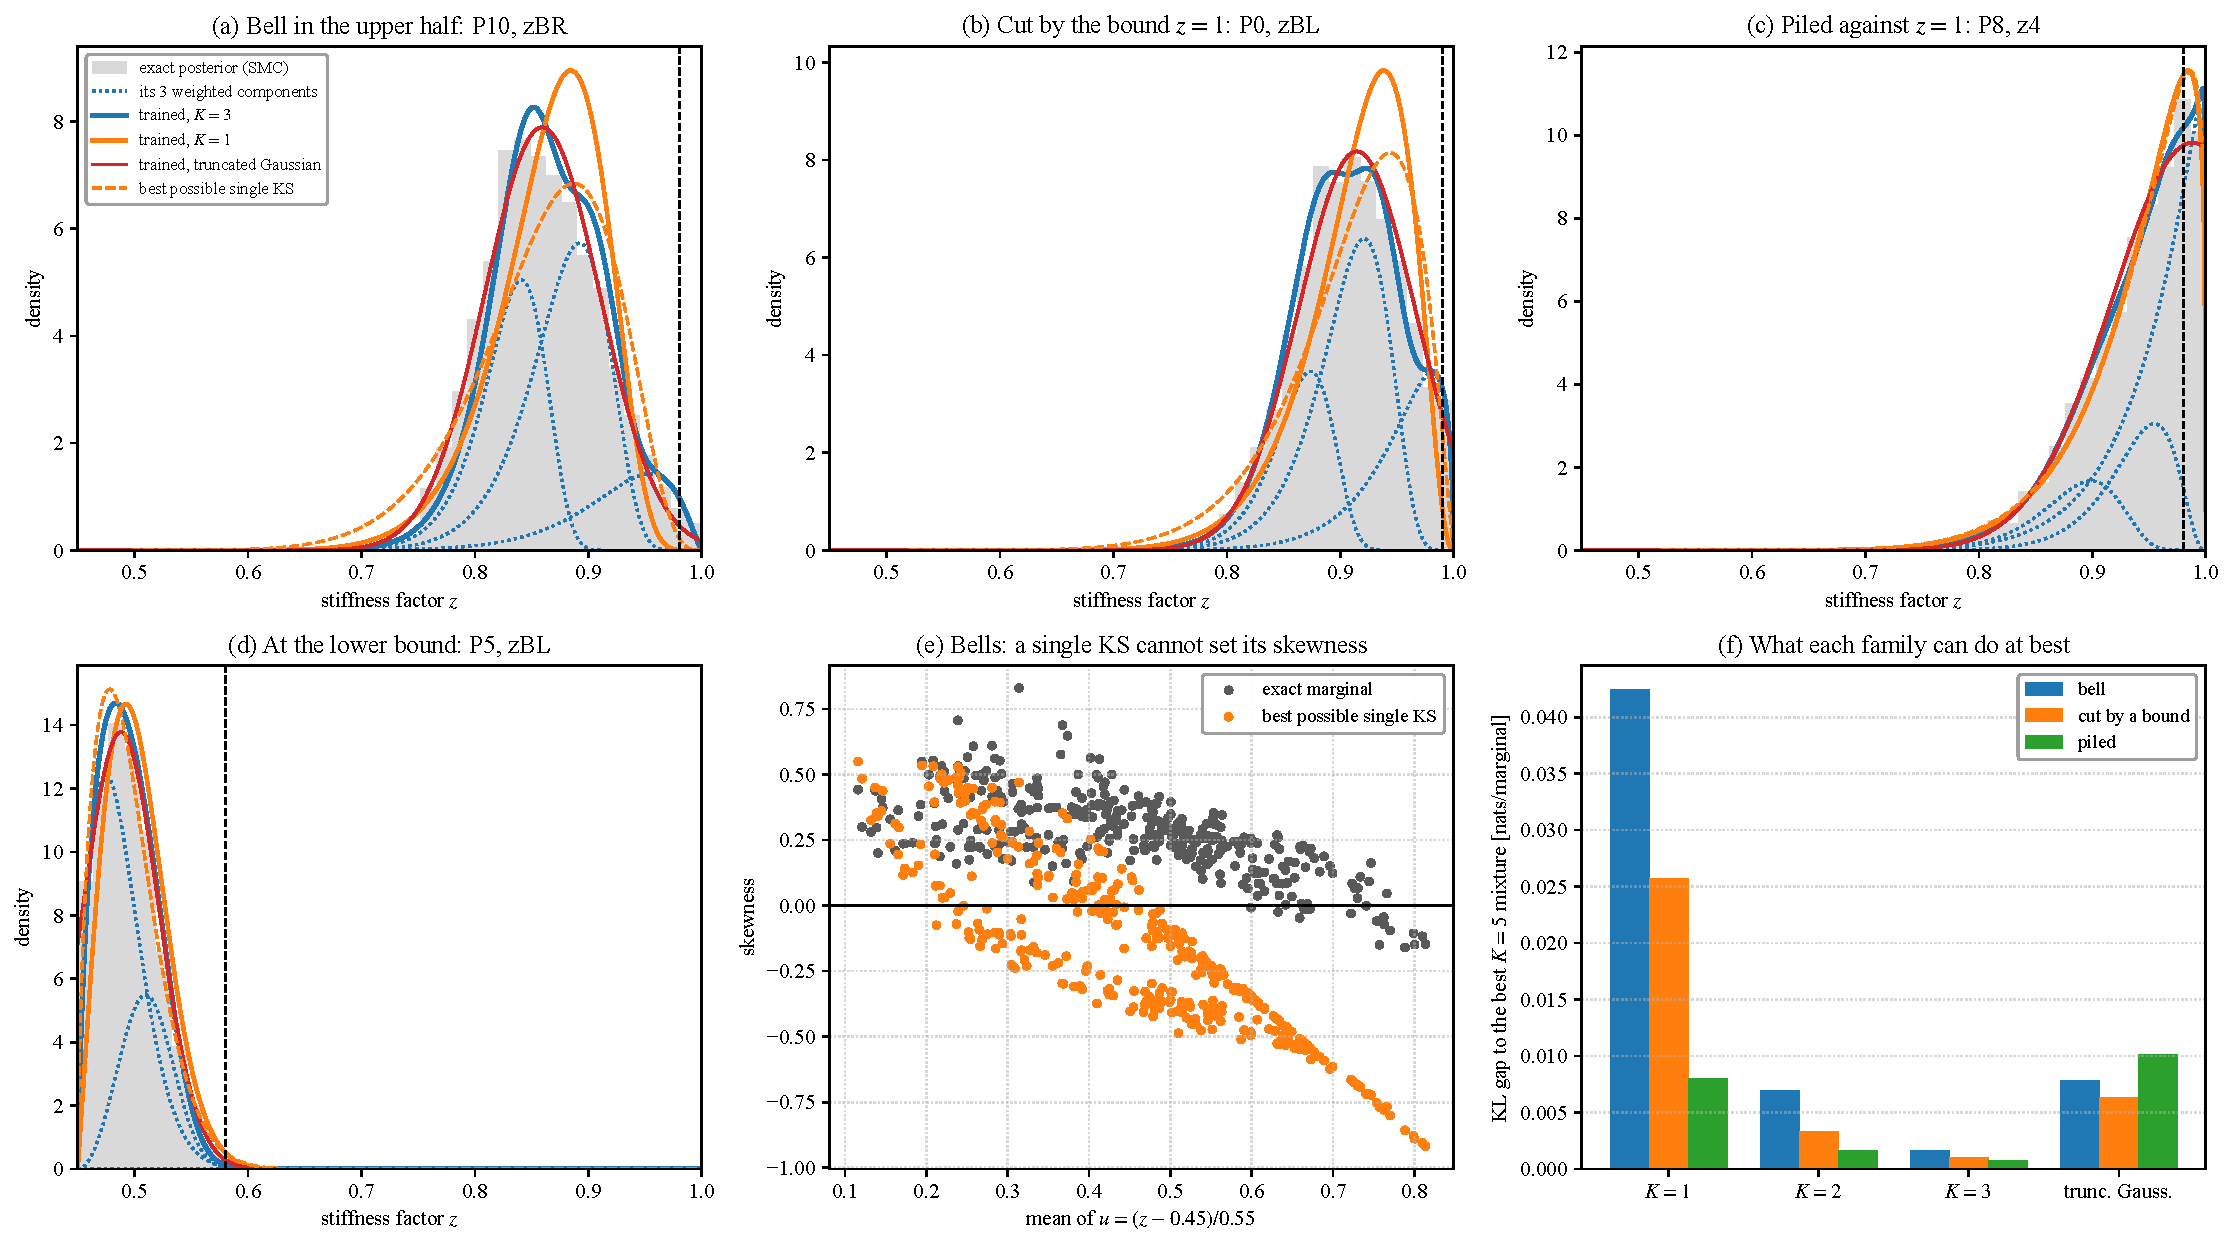
\includegraphics[width=\textwidth]{figures_results/marginal_shapes.pdf}
\caption{(a--d) Exact marginals (test set A) with the trained marginals and the best possible single Kumaraswamy; dashed
vertical line: $z^*$. Dotted: the three weighted components of the $K=3$ marginal, which overlap into one mode. (e)
Skewness of the bells: exact marginal and best single Kumaraswamy. (f) KL gap of the best member of each family.}
\label{fig:shapes}
\end{figure}

A single Kumaraswamy, $f(u)=ab\,u^{a-1}(1-u^a)^{b-1}$, has two parameters, and this limits it in two ways.
\begin{itemize}
\item \emph{Skewness.} Its location and width fix its skewness. The exact bells are right-skewed (median $+0.27$) and
nearly log-normal in $z$: the skewness of $\ln z$ is only $+0.03$, and a log-normal of the same width would have $+0.30$.
This is consistent with Eq.~(1): the logarithm of the frequencies is linear in $\ln z$ to first order. The best single
Kumaraswamy has the wrong sign as soon as the bell is in the upper part of the range, that is, for mild and moderate
damage (Fig.~\ref{fig:shapes}e). With the mean of $u$ in $[0.25,0.5)$, $[0.5,0.75)$ and $[0.75,1)$, the median skewness is
$+0.34$, $+0.20$ and $-0.10$ for the exact marginal and $-0.03$, $-0.39$ and $-0.78$ for the best single Kumaraswamy, and
its KL gap grows accordingly: 0.031, 0.064 and 0.082 nats, against 0.009 below 0.25, where the two skewnesses agree. The gap
correlates with the skewness error (0.79).
\item \emph{Bounds.} With $a,b>1$, the range of the encoder, the density vanishes at both bounds. The marginal of an
undamaged parameter is often a smooth curve cut by $z=1$, and $z^*$ lies right there. For the 242 marginals cut at $z=1$
with an interior mode, the exact density at the bound is on average 65\% of the peak. The density at $u=0.99$
relative to the peak has a median of 0.17 for the trained $K=1$, 0.62 for $K=3$ and 0.45 for GC--TN. This is where $K=1$
loses ALL on the undamaged parameters (0.970 against 1.242 in test set A; damaged: 0.608 against 0.643), and it is
visible in Fig.~\ref{fig:shapes}(a,b): $K=1$ has almost no density at $z^*$.
\end{itemize}
A single Kumaraswamy is adequate only for marginals piled against a bound (gap 0.008). A mixture removes both limits
and stays unimodal: its overlapping components build the skewness and the edge (Fig.~\ref{fig:shapes}a,b). The best
$K=2$ already reduces the gap from 0.0289 to 0.0045 nats per marginal, and the best $K=3$ to 0.0012. The truncated
Gaussian (0.0077) lies between $K=1$ and $K=2$: it is symmetric before the cut, but keeps its density at the bound. This
is why GC--TN is better than $K=1$ and worse than $K=3$ (Section~\ref{sec:baselines}).

\paragraph{How much of the deficit of $K=1$ is this.} Summed over the seven parameters of a scenario, the trained $K=1$ is
0.317 nats behind the trained $K=3$. Of these, 0.194 (61\%) is the limit of the family (best $K=3$ against best $K=1$)
and 0.123 (39\%) is a larger training gap: the trained $K=1$ falls 0.190 nats short of the best single Kumaraswamy,
whereas the trained $K=3$ falls 0.067 short of its best member and GC--TN 0.081. We do not know yet whether this larger
gap is due to the budget ($K=1$ stopped at epoch 1,142) or to the parametrization; the runs to convergence include $K=1$.
These numbers are $\mathrm{KL}(p\|q)$ of the marginals, not the $\mathrm{KL}(q\|p)$ of the joint density in the ELBO, so
they compare with Table~\ref{tab:baselines} only in order of magnitude (0.32, 0.06 and 0.18 nats per scenario for $K=1$,
GC--TN and GMM, against 0.18, 0.045 and 0.21). The best fits also suggest that $K=2$ could be close to $K=3$; it has not been
trained yet.

We do not use the multimodality rate of the supplementary metrics: the indicator, based on peaks of a kernel density
estimate of samples, has not been validated.

% =============================================================================
\section{Comparison with the baselines (R1.4)}\label{sec:baselines}
All the models share the data, decoder, likelihood, $\gamma=1$, warm-up, optimizer and budget, and differ only in the
family of $q$. Because $-\mathrm{ELBO}=\mathrm{KL}\big(q(\z|\mathbf m)\,\|\,p(\z|\mathbf m)\big)-\log p(\mathbf m)$ and
$\log p(\mathbf m)$ does not depend on $q$, the difference of mean $-$ELBO between two models on the same observations is
the difference of their mean KL divergence to the exact posterior. Table~\ref{tab:baselines} gives it with a precise
estimate (500 samples per observation, 2,400 validation observations; paired standard errors $\le0.001$ nats).

\begin{table}[t]
\centering\footnotesize
\setlength{\tabcolsep}{3.4pt}
\caption{Proposed model and baselines (one seed, 1,500-epoch budget). $\Delta$KL: mean $-$ELBO on the validation set
minus that of $K=3$, in nats per observation. KL$_{\mathrm{lb}}$: mean lower bound of $\mathrm{KL}(q\|p)$. Cov.: equal-tailed
95\% coverage. Training times depend on what else the server was running.}
\label{tab:baselines}
\begin{tabular}{l cc cc ccc cc cc}
\toprule
 & \multicolumn{4}{c}{Validation} & \multicolumn{3}{c}{Test set A} & \multicolumn{2}{c}{Test set B} & \multicolumn{2}{c}{Training} \\
\cmidrule(lr){2-5}\cmidrule(lr){6-8}\cmidrule(lr){9-10}\cmidrule(lr){11-12}
 & $\Delta$KL & KL$_{\mathrm{lb}}$ & $\hat k<0.5$ & $\hat k<0.7$ & ALL & MACE & Cov. & ALL & Cov. & best / run & s/epoch \\
\midrule
GC--KS, $K=5$    & $-0.010$ & 0.056 & 0.92 & 1.00 & 1.049 & 0.101 & 0.900 & 0.973 & 0.881 & 1,287 / 1,500 & 1.66 \\
GC--KS, $K=3$    & 0        & 0.065 & 0.89 & 0.99 & 1.044 & 0.101 & 0.900 & 0.965 & 0.883 & 1,370 / 1,500 & 1.80 \\
GC--TN (Ref.~41) & $+0.045$ & 0.110 & 0.86 & 0.99 & 1.004 & 0.119 & 0.889 & 0.911 & 0.867 & 910 / 1,210   & 1.10 \\
GC--KS, $K=1$    & $+0.182$ & 0.238 & 0.60 & 0.92 & 0.850 & 0.106 & 0.851 & 0.690 & 0.837 & 842 / 1,142   & 2.02 \\
GMM (Ref.~39)    & $+0.211$ & 0.258 & 0.54 & 0.90 & 0.915 & 0.129 & 0.855 & 0.821 & 0.839 & 1,469 / 1,500 & 1.07 \\
\bottomrule
\end{tabular}
\end{table}

The point accuracy is the same for all (MSE 0.0063--0.0064 in test set A, 0.0072--0.0073 in B); the differences are in
the uncertainty. GC--KS with $K=3$ or 5 is the closest to the exact posterior, GC--TN is 0.045 nats farther and the
GMM 0.21. These differences are for these trained models; the variability between seeds is not known yet.

\paragraph{The GMM is not collapsed, but it has one mode to fit.} All five components are used (effective number
$\exp H(\pi)$: median 4.8; mean sorted weights 0.31, 0.20, 0.18, 0.17, 0.15), and their means are at most 1.9 component
standard deviations apart (median over the test set), so they overlap into one non-Gaussian mode. This is what a mixture
should do when the target has one mode.

\paragraph{Is the budget responsible?} Not established, and the fixed budget does not allow us to say. The GMM had its
best weights at epoch 1,469, still improving slowly (median level of its validation $-$ELBO 24.033 at epoch 900 and 24.021
at epoch 1,400, with the learning rate decaying). GC--TN was stopped by noise rather than by convergence: at fixed
weights, the Monte Carlo error of the validation $-$ELBO logged during training is 0.018 nats for GC--TN against 0.006 for
GC--KS and 0.005 for the GMM, because its entropy is analytic and the error of $E_q[\mathrm{NLL}]$ is not compensated by
the sampled $\log q$. A dip of that noise at epoch 910 (recorded 23.800; level of the curve about 23.85) ended the
training at epoch 1,210 and those weights, from a learning rate of $1.7\times10^{-4}$, were restored. Runs to convergence,
with the same rule for every family and a low-noise monitor, are prepared
(\texttt{model\_comparison/run\_convergence\_gpu.sh}); they will give quality and cost separately. With the present
times per epoch, GC--TN and the GMM are about 40\% cheaper per epoch than GC--KS with $K=3$.

% =============================================================================
\section{Reviewer questions related to the results}\label{sec:reviewers}
\begin{itemize}
\item \textbf{Editor, R1.3 (under-coverage).} Equal-tailed coverage 0.900 (A), HPD 0.946; on the scenarios drawn from
the prior 0.932 (deck 0.945, bearings 0.900). The shortfall of the deck zones is a consequence of the test design
(Section~\ref{sec:coverage}). The remaining under-coverage is in the bearings; the exact posterior shows it too (0.904
on the prior scenarios), and it comes from the isotropic mode-shape term of the likelihood (Section~\ref{sec:bearings}).
\item \textbf{R1.1 (finer mesh).} The finer mesh alone changes the frequencies by at most 0.13\%; with localized damage,
test set B degrades ALL by 0.08 and coverage by 0.02, and the VAE still matches the exact posteriors
(Section~\ref{sec:testB}).
\item \textbf{R1.2, R3.1 (modelling error, mass perturbations).} Mass and stiffness deviations are present in all data
and enter the posterior through a likelihood widened by 6--9\% (frequencies) and up to 33\% (shapes). The deck
posteriors stay calibrated on the prior scenarios. The mass field also distorts the shapes of modes 4 and 5 in a
preferred direction, close to the signature of the bearings; the likelihood treats these errors as isotropic, and the
bearing posteriors become too narrow (coverage 0.90). This is how the unmodelled dynamics reach the uncertainty bounds
in this case study (Section~\ref{sec:bearings}). The size of the widening of the posteriors has not been quantified
yet (Section~\ref{sec:width}).
\item \textbf{R1.6 (healthy, mild and localized damage; false positives).} Detection rates by severity and location,
false alarms per parameter, and 11.7\% of healthy structures with at least one false alarm
(Table~\ref{tab:param}, Section~\ref{sec:width}); localized damage next to a support is hard to detect
(Section~\ref{sec:testB}).
\item \textbf{R2.2, R2.3 (bearings, damage parametrization).} The pads are the best identified parameters (posterior
std 0.04; 98\% detection for $z^*<0.75$) but have the highest false-alarm rates and under-cover, because the
likelihood over-weights the mode-shape evidence about them (Section~\ref{sec:bearings}). The zone parameter
behaves as an energy-weighted equivalent stiffness (Section~\ref{sec:testB}).
\item \textbf{R3.3 (prior and sampling density).} The DoE is not the prior. This is why coverage on the full test set
is not a calibration test (the prior itself would score 0.811), and why calibration is checked on the prior scenarios.
\item \textbf{R3.4 (number of modes).} Exact posteriors for five benchmarks: mean posterior std 0.048--0.077 with five
sensors and five modes (adopted), 0.050--0.070 with four modes, 0.063--0.090 with three modes and 0.069--0.103 with
three sensors and three modes; widest 95\% interval 0.27--0.42, 0.25--0.46, 0.36--0.50 and 0.37--0.52. With fewer modes
a left--right ambiguity appears: in P1 ($z_1$ damaged) the posterior probability that the mirror zone $z_5$ is damaged
($z_5<0.85$, the threshold of that study) is 0.07, 0.16, 0.34 and 0.51. Each value comes from a single observation and is noisy (with seven sensors and five
modes it is 0.33). VAE results with three modes are pending.
\item \textbf{R3.8, R1.7 (cost).} One training takes 0.64--0.75~h (1,142--1,500 epochs, 1.7--2.0~s per epoch) on one
GPU; the GPU model must still be reported. We have not timed the inference.
\item \textbf{R3.2 ($\gamma$).} $\gamma=1$ in all runs; $K$ is chosen on the validation set; the test sets were used
once.
\item \textbf{R1.4 (comparison with Refs.~39 and 41).} Same point accuracy; GC--KS with $K=3$ is 0.045 nats closer to the
exact posterior than GC--TN and 0.21 nats closer than the GMM, at about 1.6 times their time per epoch
(Section~\ref{sec:baselines}). Preliminary: one seed and a fixed budget; runs to convergence are prepared.
\item \textbf{Pending:} R1.5 (out-of-distribution sets).
\end{itemize}

% =============================================================================
\section{What we do not know yet}\label{sec:open}
\begin{enumerate}
\item Whether a full covariance of the shape residuals restores the coverage of the bearings (Section~\ref{sec:bearings}).
Check: exact posteriors of the 120 prior scenarios under that likelihood, a few minutes; only then decide whether to
retrain with it.
\item Why the copula term at $z^*$ is close to zero, instead of positive, on the prior scenarios.
\item Whether $K=5$ improves on $K=3$ (one seed only; multi-seed study running).
\item Whether the larger training gap of $K=1$ (Section~\ref{sec:shapes}) is due to its budget or to the parametrization,
and whether $K=2$ is close to $K=3$ once trained.
\item How much the modelling error widens the posteriors with respect to noise only. Check: exact posteriors of the
benchmarks under the calibrated and the noise-only likelihoods.
\item How much of the gap between the families remains after training to convergence, and at what cost.
\end{enumerate}

\end{document}
